\documentclass{cheat-sheet}

\pdfinfo{
  /Title (Zusammenfassung Markovketten)
  /Author (Tim Baumann)
}

\usepackage{bbm} % Für 1 mit Doppelstrich (Indikatorfunktion)
\usepackage{mathtools} % psmallmatrix environment
\usepackage{nicefrac}

\usepackage{tikz}
\usetikzlibrary{matrix}

% Kleinere Klammern
\delimiterfactor=701

% TODO: Include-File für Stochastik

\newcommand{\Alg}{\mathfrak{A}} % (Mengen-)Algebra
\renewcommand{\P}{\mathbb{P}} % Wahrscheinlichkeitsmaß
\newcommand{\E}{\mathbb{E}} % Erwartungswert
\newcommand{\ind}{\mathbbm{1}} % Indikatorfunktion
\newcommand{\iid}{i.\,i.\,d.} % identisch unabhängig verteilt

\DeclareMathOperator{\var}{Var} % Varianz
\DeclareMathOperator{\cov}{Cov} % Kovarianz
\DeclareMathOperator{\cor}{Cor} % Korrelation

\begin{document}

\raggedcolumns % stretche Inhalt nicht über die gesamte Spaltenhöhe

\maketitle{Zusammenfassung Markovketten}

% Vorlesung vom 4.5.2017

% Kapitel II. Abzählbare Markovketten
\section{Abzählbare Markovketten}

% §2.1. Rekurrenz und Transienz

\begin{nota}
  Sei im Folgenden $\{ Z_n \}$ eine Markovkette auf einem abzählbaren Zustandsraum~$E$.
\end{nota}

% 2.1
\begin{defn}
  Für $x \in E$ definiere die Zufallsvariablen
  \[ \begin{array}{r l}
    \tau_x^{(1)} & \coloneqq \inf \Set{n > 0}{Z_n = x} \in \N \cup \{ \infty \} \\
    \tau_x^{(k)} & \coloneqq \inf \Set{n > \tau_x^{(k-1)}}{Z_n = x}, \enspace k > 1.
  \end{array} \]
  (Beachte: $\tau_x^{(k)}$ ist eine messbare Abbildung.)
\end{defn}

\begin{bem}
  Ferner gilt $\{ \tau_x^{(k)} = n \} \in \sigma(Z_0, Z_1, \ldots, Z_n)$.
\end{bem}

\begin{defn}
  Für $x, y \in E$ sei
  $F(x, y) \coloneqq P(\tau_y^{(i)} < \infty \mid Z_0 = x)$
\end{defn}

% 2.2
\begin{lem}
  Für alle $x, y \in E$ und $k \geq 1$ gilt
  \[ P(\tau_y^{(k)} < \infty \mid Z_0 = x) = F(x, y) \cdot F(y, y)^{k-1}. \]
\end{lem}

\begin{nota}
  $\tilde{\ell}(y) = \sum_{k=j}^\infty \ind \{ Z_k = y \}$
\end{nota}

Dann gilt $P(\tau_y^{(k)} < \infty \mid Z_0 = x) = P(\tilde{\ell} \geq k \mid Z_0 = x)$

% 2.3
\begin{defn}
  Ein Zustand $x \in E$ heißt
  \begin{itemize}
    \item \emph{absorbierend}, falls $p(x, x) = 1$,
    \item \emph{rekurrent}, falls $F(x, x) = 1$ und
    \item \emph{transient}, falls $F(x, x) < 1$.
  \end{itemize}
\end{defn}

\begin{bem}
  Absorbierende Zustände sind rekurrent.
\end{bem}

% ausgelassenes  Beispiel: a+1 Zustände nebeneinander, der linke und rechte sind absorbierend, die dazwischen haben eine Übergangswahrscheinlichkeit von 1/2 nach links und 1/2 nach rechts

% ausgelassenes Beispiel: Irrfahrt auf \N
% Falls $p \leq \nicefrac{1}{2}$, so ist Anfangszustand rekurrent
% Falls $p > \nicefrac{1}{2}$, so ist Anfangszustand transient
% Parondo-Paradoxon

\begin{bsp}
  In der Markovkette
  \begin{center}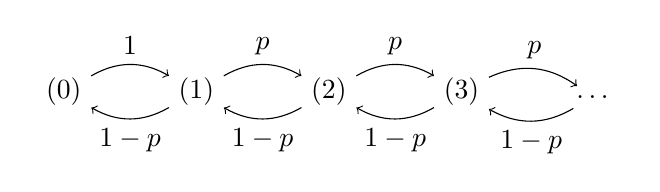
\begin{tikzpicture}
    \matrix [matrix of nodes, column sep=1cm, row sep=0.8cm] {
      \node (N0) {(0)}; &
      \node (N1) {(1)}; &
      \node (N2) {(2)}; &
      \node (N3) {(3)}; &
      \node (N4) {\ldots}; \\
    };
    \draw[->, bend left=30] (N0) to node [above] {$1$} (N1);
    \draw[->, bend left=30] (N1) to node [below] {$1 - p$} (N0);
    \draw[->, bend left=30] (N1) to node [above] {$p$} (N2);
    \draw[->, bend left=30] (N2) to node [below] {$1 - p$} (N1);
    \draw[->, bend left=30] (N2) to node [above] {$p$} (N3);
    \draw[->, bend left=30] (N3) to node [below] {$1 - p$} (N2);
    \draw[->, bend left=30] (N3) to node [above] {$p$} (N4);
    \draw[->, bend left=30] (N4) to node [below] {$1 - p$} (N3);
  \end{tikzpicture}\end{center}
  ist (0) genau dann rekurrent, falls $p \leq \nicefrac{1}{2}$, ansonsten transient.
  \TODO{genauer!}
\end{bsp}

% 2.6
\begin{defn}
  Für $y \in E$ sei
  \[
    \ell(y) \coloneqq \sum_{k=0}^\infty \ind \{ Z_k = y \}
  \]
  die \emph{Anzahl der Besuche in~$y$}.
  Die \emph{Green'sche Funktion} von $\{ Z_n \}$ ist $G : E \times E \to \cinterval{0}{\infty}$ mit
  \[
    G(x, y) \coloneqq \E(\ell(y) \mid Z_0 = x).
  \]
\end{defn}

\begin{bem}
  $G(x, y) = \E \left( \sum_{k=0}^\infty \ind \{ Z_k = y \} \mid Z_0 = x \right) = \sum_{k=0}^\infty P(Z_k = y \mid Z_0 = x) = \delta_{xy} + \sum_{k=1}^\infty p^{(k)}(x, y)$
\end{bem}

% 2.7
\begin{satz}
  Für alle $x, y \in E$ gilt
  \[
    G(x, y) = 
    \begin{cases}
      \tfrac{F(x, y)}{1 - F(y, y)} & \text{falls $x \neq y$}, \\
      \tfrac{1}{1 - F(y, y)} & \text{falls $x = y$}. \\
    \end{cases}
  \]
\end{satz}

\begin{kor}
  $x$ ist rekurrent $\iff$ $G(x, x) = \infty$
\end{kor}

% 2.8
\begin{satz}
  ist $x \in E$ rekurrent und $F(x, y) > 0$, so ist $y$ auch rekurrent und $F(x, y) = F(y, x) = 1$.
\end{satz}

\iffalse
% 2.9
\begin{interp}
  %Die Aussage kann man wie folgt deuten:
  $F(x, y) > 0$ bedeutet, dass nach jedem Besuch in~$x$ der Zustand $y$ auch besucht wird mit positiver Wahrscheinlichkeit und die Rekurrenz von~$x$ bedeutet, dass $x$ unendlich oft besucht wird.
  Der Satz sagt, dass dann auch $y$ unendlich oft besucht wird.
\end{interp}
\fi

% 2.9
\begin{bem}
  $F(x, y) > 0 \iff \ex{n \geq 1} P^{(n)}(x, y) > 0$
\end{bem}

% 2.10
\begin{defn}
  $\{ Z_n \}$ heißt \emph{irreduzibel}, falls $\fa{x, y \in E} F(x, y) > 0$.
\end{defn}

% 2.11
\begin{satz}
  Sei $\{ Z_n \}$ irreduzibel.
  Dann sind entweder alle Zustände rekurrent oder alle Zustände transient.
\end{satz}

% Vorlesung vom 9.5.2017

% 2.12
\begin{satz}
  Eine irreduzible Kette auf einem endlichen Raum ist immer rekurrent.
\end{satz}

% §2. Rekurrenz und Transienz von Irrfahrten
\section{Rekurrenz und Transienz von Irrfahrten}

Sei $\{ Z_n \}$ eine Irrfahrt auf $\Z^d$, \dh{} $p(x, y) = p(0, y - x) =: q(y - x)$.

Mit anderen Worten: Die Zuwächse $\{ Z_n - Z_{n-1} \}_{n \geq 1}$ sind \iid{} Zufallsvariablen.

\begin{bsp}
  Einfache Irrfahrt auf~$\Z$:
  $p(0, 1) = p$, $p(0, -1) = q = 1 - p$
\end{bsp}

%Für welche Werte von $p$ ist diese Irrfahrt rekurrent/transient?

In diesem Fall kann man die Greensche Funktion exakt berechnen:

\begin{align*}
  G(x, x) = G(0,0) = \sum_{m=0}^\infty p^{(m)}(0, 0) = 1 + \sum_{n=1}^\infty p^{(2n)}(0, 0) = 1 + \sum_{n=1}^\infty \binom{2n}{n} p^n (1-p)^n
  = 1 + \sum_{n=1}^\infty \binom{2n}{n} 4^{-n} (4 p (1-p))^n = (1 - 4 p (1-p))^{-\tfrac{1}{2}} = \tfrac{1}{\abs{2p - 1}}
\end{align*}

% 2.13
\begin{satz}
  Sei $\{ Z_n \}$ eine Irrfahrt auf~$\Z$ mit $\E \abs{Z_1 - Z_0} = \sum_{x \in \Z} \abs{x} p(0, x) < \infty$.
  Dann gilt
  \[
    \{ Z_n \} \text{ ist rekurrent} \iff \sum_{x \in \Z} x p(0, x) = 0.
  \]
\end{satz}

\begin{defn}
  Einfache symmetrische Irrfahrt auf $\Z^d$ ist eine translationsinvariante Markovkette mit $p(0, \pm e_i) = \tfrac{1}{2 d}$ für $i = 1, \ldots, d$.
\end{defn}

Für einfache symm. Irrfahrten gilt:
$p^{(2n)}(x, x) = \sum_{k_1, \ldots, k_d \in \N, k_1 + \ldots + k_d = n} \tfrac{(2n)!}{(k_1!)^2 \cdot (k_d!)^2} (\tfrac{1}{2d})^{2n}$

Für $d = 2$ gilt $p^{(2n)}(0, 0) = [\binom{2n}{n} (\tfrac{1}{2})^{2n}]^2$

Mit der Stirling'schen Formel folgt $p^{(2n)}(0, 0) \approx \tfrac{1}{\pi n}$.

Somit gilt $\sum p^{(2n)}(0,0) = \infty$.

\begin{fazit}
  Die zweidimensionale einfache symm. Irrfahrt ist rekurrent.
\end{fazit}

% Vorlesung vom 11.5.2017

\begin{bem}
  Man kann zeigen:
  Für einfache symm. Irrfahrten auf~$\Z^d$ gilt:
  \[ p^{2n}(0,0) \leq \tfrac{C_d}{n^{\nicefrac{d}{2}}} \]
  Somit ist die einfache Irrfahrt transient für alle $d \geq 3$.
\end{bem}

\begin{defn}
  $\varphi(t) \coloneqq \sum_{x \in \Z^d} e^{i (t \cdot x)} p(0, x)$ für $t \in \R^d$
\end{defn}

Da die Zuwächse $\{ Z_n - Z_{n-1} \}$ \iid{} sind, so gilt
\[ \sum_{x \in \Z^d} e^{i (t \cdot x)} p^{n}(0, x) = \varphi^n(t), \quad n \geq 1 \]

Inversionsformel: $p^{n}(0, x) = \tfrac{1}{(2 \pi)^d} \int{\cointerval{-\pi}{\pi}^d}{}{e^{- i (t \cdot x)} \varphi^n(t)}{t}$

\begin{satz}
  Für jede Irrfahrt $\{ Z_n \}$ auf $\Z^d$ gilt
  \[ G(0, 0) = \left( \tfrac{1}{2 \pi} \right)^d \lim_{\lambda \uparrow 1} \int{t \in \cointerval{-\pi}{\pi}^d}{}{Re(\tfrac{1}{1 - \lambda \varphi(t)})}{t} = \infty \]
\end{satz}

\begin{bsp}
  Für die einfache symm. Irrfahrt $\{ Z_n \}$ auf~$\Z^d$ ist
  \[
    \varphi(t) = \tfrac{1}{d} \sum_{k=1}^d \cos(t_k)
  \]
  Mit der Ungleichung $1 - \cos(u) \geq c_0 u^2$ für alle $u \in \cinterval{- \pi}{\pi}$ folgt
  \[
    \varphi(t) \geq \tfrac{c_0}{d} \abs{t}^2.
  \]
  Es folgt
  \[
    \tfrac{1}{1 - \lambda \varphi(t)} \leq \tfrac{d}{\lambda c_0} \abs{t}^{-2}
  \]
  Die Funktion $\abs{t}^{-2}$ ist auf $\cointerval{-\pi}{\pi}^d$ für jedes $d \geq 3$ integrierbar.
  Somit ist die einfache Irrfahrt auf $\Z^d$, $d \geq 3$, transient.
\end{bsp}

% 2.16
\begin{satz}
  Jede irreduzible Irrfahrt auf $\Z^d$ mit $d \geq 3$ ist transient.
\end{satz}

% 2.17
\begin{bsp}
  Sei $\{ Z_n \}$ eine Irrfahrt auf $\Z$ mit $p(0, x) = p(0, -x)$.
  Angenommen $x^\alpha p(0, x) \to c \in \ointerval{0}{\infty}$ für $x \to \infty$ für ein $\alpha > 1$.
  Dann gilt
  \[ 1 - \varphi(t) = \sum_{n=-\infty}^\infty (1 - \cos(nt)) p(0, n) \]
  und
  \[
    \tfrac{1 - \varphi(t)}{\abs{t}^{\alpha - 1}} = \sum_{n=-\infty}^\infty \abs{n}^\alpha p(0, n) \abs{t} f(n t)
  \]
  mit $f(x) = \tfrac{1 - \cos(x)}{\abs{x}^\alpha}$.
  Außerdem $\abs{n}^\alpha p(0, n) = c + \epsilon_n$, wobei $\epsilon_n \to 0$ für $\abs{n} \to \infty$.
  Es folgt
  \[
    \tfrac{1 - \varphi(t)}{\abs{t}^{\alpha - 1}} = \sum_{n=-\infty}^\infty c \abs{t} f(n t) + \sum_{n=-\infty}^\infty \epsilon_n \abs{t} f(n t).
  \]
  Für $t \to 0$ hat man
  \[ \sum_{n=-\infty}^\infty \abs{t} f(n t) \to \int{-\infty}^{\infty}{f(x)}{x} \]
  und
  \[ \sum_{n=-\infty}^\infty \epsilon_n \abs{t} f(n t) \to 0. \]
  Es folgt für $\alpha < 3$
  \[ \lim_{t \to 0} \tfrac{1 - \varphi(t)}{\abs{t}^{\alpha - 1}} = c \int{-\infty}{\infty}{\tfrac{1 - \cos(x)}{\abs{x}^\alpha}}{x} < \infty \]
  Folglich ist $\tfrac{1}{1 - \varphi(t)}$ für $\alpha < 2$ integrierbar und somit $\{ Z_n \}$ transient.
  Für $\alpha = 2$ ist $\tfrac{1}{1 - \varphi(t)}$ in der Umgebung von null nicht integrierbar und damit $\{ Z_n \}$ rekurrent.
  Für $\alpha > 2$ ist $\sum \abs{x} p(0, x) < \infty$ und somit ist die Irrfahrt rekurrent, da der Erwartungswert der Zuwächse null ist.
\end{bsp}

\end{document}